\chapter{Implementation}
\section{Design}
	Now that we had shown that a classifier could be built with relatively small sets of training data that still performed well, we had to design the interface to expose this functionality. This largely involved assessing tradeoffs between choices.
	
	\subsection{`Sketchy' or Formal}	
	\begin{figure}[h]
		\centering
		\begin{subfigure}[b]{0.4\textwidth}
			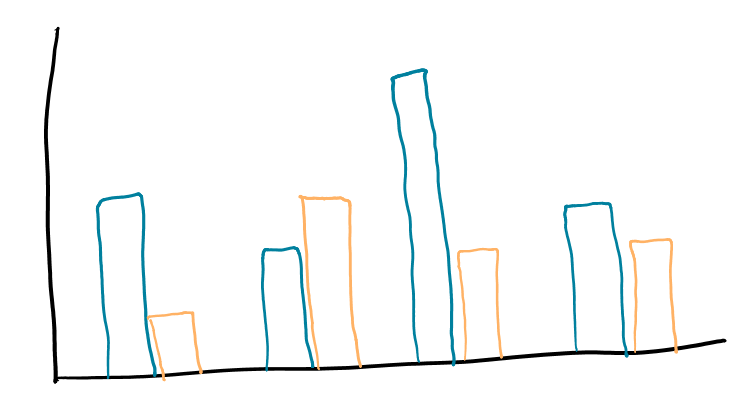
\includegraphics[width=\textwidth]{sketchy}
			\caption{Sketchy look}
			\label{fig:sketchy}
		\end{subfigure}
		\begin{subfigure}[b]{0.4\textwidth}
			\includegraphics[width=\textwidth]{formal}
			\caption{Formal look}
			\label{fig:formal}
		\end{subfigure}
	\end{figure}
	User content can be in shown in two styles: sketch or formal. \citep{yeung_effect_2008} showed that a doodle-like appearance encourages early-stage experimentation and discussion, whereas a formal appearance looks finished and professional. Thus, we had to choose whether the system should generate the rest of the chart with a 'sketchy' look, or convert the input into a finished chart with a formal look. Generating the 'sketchy' look can be non-trivial, \citep{plimmer_sketchnode:_2010, wang_sketchset:_2011} e.g.\ if the user draws one bar, how should the system generate more bars that look hand-drawn by the same author but not just like stretched versions of the first bar? Additionally, if the users want to present these charts to an audience, they must look polished, and so at some point an export option for a formal look needs to be offered. Thus, we decided to offer a hybrid that shows the user's input in sketch form, but also the formal chart generated by the system.
	
	%TODO Gestures or sketches	
	% Can cite Chao
	\subsection{Modes or modeless}
	Since the application now has both sketch and formal content, the user must have an easy way to switch between the two views. One approach is to give the user an explicit UI widget to toggle between the two modes. This way, the user explicitly indicates what they want to see, and thus should have a better understanding of what state the system is in. This also allows the system a chance to change the controls available to the user.
	
	The other approach is to avoid modes, requiring lesser cognitive effort from the user since they don't need to keep track of what state the system is in. In this project, this could have been done by showing the sketch view when the user was about to edit the chart. The active digitizer hardware allows the system to detect when the user brings the stylus within range of the screen, just before they actually touch the screen, allowing the chart to be in sketch view by the time the stylus is down. When the stylus goes out of range, the system can switch to the formal chart view. This would solidify the metaphor that edits are done to the sketch, but the final product to be looked at is the formal view. 
	
	At first, the modeless version was chosen for its lower cognitive overhead. However, when the extension to allow edits not just to the sketch view, but also the formal view, was undertaken, we had to switch over to a mode-based system to allow the user to interact with the graph in both views with their stylus.
	
	\subsection{Standard or custom charting}	
	Since the system is generating a formal version of the chart, a charting component is required to render this visualisation. The .NET framework comes with built-in chart controls that offer basic functionality with relatively low implementation effort. They also allow easy export as dynamic chart objects into Microsoft Office files. However, customising their appearance beyond a certain point is extremely difficult, making it easier to just make one's own charting component from scratch and control all aspects of the rendering. This means having to re-implement a lot of core functionality though, such as scaling shapes correctly, choosing labels that are round figures when possible, and generating colours than work well together for different data series. This also means that the chart can only be exported as a raster image rather than as a chart object.
	
	To enable rapid prototyping, we chose to utilise the standard charting component at first. As our needs to customise the chart grew, we were able to make our own chart class that implemented the same interface as the standard component, and so could be slotted in to replace it.
	
	\subsection{Finite or infinite domain}
	Some tools, such as Microsoft Excel, let the user make one of a limited set of charts, such as bar or pie charts, quickly. Others, (which usually involve coding), such as D3.js, let the user make a vast variety of visualisations by creatively combining basic elements like lines, boxes and wedges. However, these require expert knowledge of the tools, and take longer to create basic visualisations. 
	
	\begin{table}[h]
	\begin{tabular}{p{0.5 \linewidth} p {0.5 \linewidth}}
	\bfseries Library of charts 	& \bfseries Modular charts \\
	Draw basic gestures or elements to indicate which chart type is desired & Draw any one of 7 basic components (lines, bars, labels etc) and bind data to attributes of theirs such as width, height, colour or radius \\
	Finite domain 		& Infinite domain \\
	Quick				& Slower \\
	Simple interface, just drop data on an element to bind data	& Complex interface to expose all attributes and manage data binding \\
	\end{tabular}
	\end{table}
	
	\citep{chao_poster:_2010} uses pen gestures to indicate 'proto-objects' that can be combined. While an infinite domain system that uses pen sketches would have been intriguing to explore, it would contradict the project's primary usability goal that the system should be faster than users' current systems. Additionally, the 80/20 rule indicated that while a few power users may want to generate custom visualisations, the majority would just want to make simple charts. Thus, the additional functionality didn't justify the additional complexity for the average user.
	
%	\subsection{To beautify or not to beautify}
%	The formal graphics generated by the system are easy to modify with existing tooling, whereas human ink strokes are less straightforward to modify while maintaining their natural look and feel.


	\section{Development}
		At a high level, the program is composed of 3 components - data handling, sketch processing and charting (in increasing order of complexity). It is written in an Object Oriented fashion, with separation between the views (Windows Forms) and controllers (C\# classes), to allow for easy testing.
	\subsection{Data import and management}
		Since the application is targeted at the average user, their data is most likely to be stored in spreadsheet format. Thus, it is important to allow them to import data from .xlsx and .csv files. 
		For the sake of simplicity, the code assumes that the data is well-formed. Specifically, it works on the following assumptions:
		\begin{enumerate}
		\item The data is arranged as records in the rows of the spreadsheet.
		\item The first row contains the names of the various fields.
		\item No data is missing (if there are $m$ columns and $n$ rows, there are $m \cdot n$ data values.
		\end{enumerate}
		
		Under these assumptions, importing tabular data is a common use case, so I studied a number of existing libraries and methods to do this in C\# and ultimately settled on built-in OLE data import functionality. 
	\subsection{Sketch Processing Workflow}
	\subsection{Charting}
	